\section{Frekvensgenerator}\label{sec:frekv_gen}
I dette afsnit vil alle overvejelser omkring frekvensgeneratoren blive gennemgået, hertil designvalg og beregninger. 
\subsection{Design}
Til at generere et signal ud fra batterierne anvendes en timer-kreds. 
Timeren skal her bruges til at lave et puls-signal, der har en given frekvens og duty-cycle, i dette projekt et firkantsignal. 
Der er her valgt en konfiguration der hedder A-stable. 
Fordelen ved dette er at timeren kan hente sit input direkte fra forsyningen der i dette tilfælde er et batteri. Dette koster en ekstra modstand men har den fordel, at duty-cycle og frekvens bliver frie variabler. 
Dette signal skal have en frekvens, der er tilpas høj, så systemet er mindre modtagelig overfor forstyrrelser, og det vil samtidig give en hurtigere responstid. 

Outputsignalet fra timeren er begrænset således, at udgangsspændingen kun kan antage positive værdier.
For at løse dette, sættes en kondensator i serie med spolen.
Det gør at spolen bliver påtrykt en spænding af varierende polaritet, hvilket også giver et konstant skiftende magnetfelt.
\begin{figure}[h!]
	\centering
	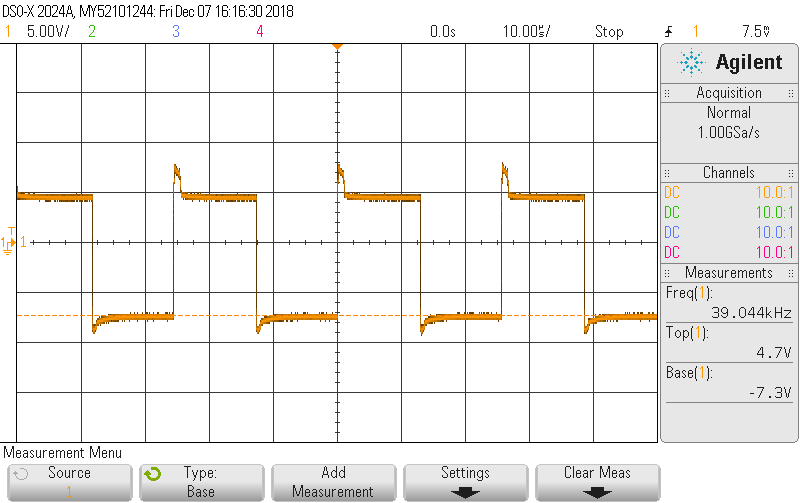
\includegraphics[width=1\textwidth]{billeder/freq_png.png}
	\caption{Her ses outputtet fra frekvensgeneratoren}
	\label{fig:frekvensgenerator}
\end{figure}
Inden kredsløbet tegnes færdigt skal der tages højde for den spænding timeren leverer. 
Spolen har en meget lille indre modstand, hvilket medfører at ved høje spændinger, skal timeren levere en stor strøm. 
Da timeren ikke kan holde til at levere mere end $225 \si{\milli\ampere}$, sættes en modstand i serie for at begrænse strømmen. 
Det færdige kredsløb ses på figur \husk{Kenneth}{indsættelse af figur}

\subsection{Beregninger af komponenter}
Til udregning af modstandens og kondensatorens værdier anvendes to af de ligninger der er opgivet i databladet for NE555 timeren. 
Først anvendes ligning 5 i databladet til at bestemme modstanden $R_5$. 
Da der ikke er ligninger nok, bliver duty-cyclen og modstanden $R_6$ valgt. 
Duty-cyclen sættes til $D = 51\%$  , og $R_6$ vælges til$ 15\si{\kilo\ohm}$. 
Ligning 5 \cite[Side 11.]{NE555} i databladet omskrives svarende til i ligning \ref{eq:TimerInputModstand}.
\begin{align}
R_5 & = \frac{R_6}{D} - 2 \cdot R_6 \label{eq:TimerInputModstand}
\end{align}
Parametrene indsættes i ligning \ref{eq:TimerInputModstand}.
Resultatet viser her at $R_5$ skal være $588\si{\ohm}$ for at opnå en duty-cycle på $51\%$ .
Som det sidste skal der udregnes en kondensator der forbindes til trigger indgangen og til ground. 
Til dette anvendes ligning 4 i databladet \cite[Side 11]{NE555}. Denne ligning isoleres for kondensatoren som givet i ligning \ref{eq:Kondensator_c7}.
Modstandsværdierne er kendte, og der bestemmes her for en frekvens på $F_n = 50 \si{\kilo\hertz}$.
\begin{align}
	C_7 & = \frac{1}{F_n \cdot \left( \frac{25 \cdot R_5 }{36} + \frac{25 \cdot R_6}{18} \right) \label{eq:Kondensator_c7}}
\end{align}
Ud fra ligning \ref{eq:Kondensator_c7} fås en kondensator værdi på $C_7 = 0.9\si{\nano\farad}$ for at få en frekvens på 50 \si{\kilo\hertz}. 
Da disse størrelser ikke kan realiseres i de lagerførte SMD værdier, vælges derfor tilnærmede værdier. 
Dette medfører at $R_5$ bliver $680\si{\ohm}$ og $C_7$ på $1\si{\nano\farad}$. 
Heraf udregnes duty-cycle og frekvens ved at bruge ligning 4 og 5 i databladet. \cite[Side 11.]{NE555}

Dette giver en duty-cycle på $D = 49\%$ og en frekvens $F_n = 46.9\si{\kilo\hertz}$. 
Duty-cyclen ligger tæt på $50\%$ og den ønskede frekvens er stadig stor nok til at en lille afvigelse ikke kommer til at have en væsentlig betydning. Denne opstilling accepteres.

Der skal herefter sættes en kondensator på udgangen, således at udgangsspændingen kan antage både positive og negative værdier. 
Middelspændingen over en spole er $0\si{\volt}$, men det er outputtet ikke, da den ikke oscillerer omkring $0 \si{\volt}$, hvilket er kondensatorens formål. 
\subsection{Beregning af udgangskondensator}
For at kunne finde afsenderspolens impedans, anvendes vinkelfrekvensen $\omega_c$ som udregnes i ligning \ref{eq:vinkelfrekvens}.
\begin{align}
	\omega_c & = 2 \cdot \pi \cdot F_n \label{eq:vinkelfrekvens}
\end{align}
Der fås en vinkelfrekvens på $\omega_c = 294.910\si{\kilo\radian\per\second}$.
Afsenderspolens induktans måles ved hjælp af en RLC-meter til $L = 205\si{\micro \henry}$.
Det ønskes ikke at spolens impedans bliver lige så stor som kondensatorens, idet der så opstår en resonanskreds. 
Spolens impedans udregnes ved ligning \ref{eq:impedans2}.

Den udregnede impedans er $Z_L = 60.5 \si{\ohm}$.
Der vælges her at spolens impedans skal være 20 gange større end kondensatorens impedans. Størrelsen på kondensatoren udregnes ved ligningen \ref{eq:kondensator_c9}.
\begin{align}
	Z_{C9} & = \frac{20}{\omega_c \cdot C_9} \rightarrow C_9 = 1.1 \si{\micro\farad} \label{eq:kondensator_c9}
\end{align}
Ved en kondensator størrelse på $1.1\si{\micro\farad}$ er størrelsesforholdet mellem de 2 impedanser 20 gange. 
SMD kondensatoren der passer til er på $1\si{\micro\farad}$. Det praktiske størrelsesforhold udregnes igen hvor $C_9 = 1\si{\micro\farad}$. Størrelsesforholdet bliver da $\si{Z_L \per Z_{C9}} = 17.8$ gange, hvilket er acceptabelt.

På grund af modstanden og kondensatoren i kredsløbet, opstår der en forsinkelse i systemet, der er lig produktet af kondensatoren $C_9$ og modstanden $R_7$. $R_7$ er et potentiometer, så i beregningen anvendes højeste værdi, som er $1\si{\kilo\ohm}$.
\begin{align}
	\tau & = R \cdot C = 1 \si{\milli\second}
\end{align}
Forsinkelsen på $1 \si{\milli\second}$ er acceptabelt for systemet.

